% ACM sigconf — Cloud Forensics Bangladesh
% Figures recreated with TikZ from original PDF
\documentclass[sigconf,nonacm]{acmart}

%% ── Packages ──────────────────────────────────────────────────────────────
\usepackage{tikz}
\usetikzlibrary{shapes.geometric, shapes.misc, arrows.meta, positioning,
                fit, backgrounds, calc}
\usepackage{booktabs}
\usepackage{array}
\usepackage{tabularx}
\usepackage{microtype}
\usepackage{balance}
\usepackage{enumitem}
\setlist[itemize]{leftmargin=*,noitemsep,topsep=2pt}

%% ── Metadata ──────────────────────────────────────────────────────────────
\title{Cloud Forensics Challenges in Bangladesh: A PRISMA Systematic Review
       with AI-Enhanced Resolution Strategies}

\author{Md.\ Ahsan Kabir}
\affiliation{%
  \institution{United International University}
  \department{Department of Computer Science and Engineering}
  \city{Dhaka}
  \country{Bangladesh}}
\email{mkabir2520016@mscse.uiu.ac.bd}

\begin{abstract}
Bangladesh's accelerating cloud adoption---over 100 million
internet-enabled devices and more than \$1.2 billion in public-sector
cloud procurement since 2020---has outpaced the legal and procedural
infrastructure governing digital investigations. The country's
investigative statutes (ICT Act 2006, Digital Security Act 2018, Cyber
Security Act 2023) were drafted for physical endpoint devices and are
silent on cloud-hosted evidence, statutory log preservation, and
cross-border jurisdictional complexity. The result is a growing gap: the
Cyber Tribunal records a disproportionately high acquittal rate on
cloud-sourced evidence cases, driven not by disputed facts but by
chain-of-custody failures and Section~65B admissibility deficiencies.

This paper addresses that gap through a PRISMA 2020-compliant review of
16 open-access publications (2021--2026), identifying five challenge
clusters (C1--C5) and mapping each to a validated AI resolution strategy
with quantitative evidence. The resulting
\emph{AI-Enhanced Cloud Forensic Readiness Framework for Bangladesh}
(AI-CFRF-BD) provides a phased, locally implementable pathway for
Bangladesh's law enforcement and policymakers.
\end{abstract}

\keywords{cloud forensics, digital evidence, Bangladesh cyber law, PRISMA
systematic review, AI forensics, blockchain chain-of-custody}

%% ── TikZ styles ──────────────────────────────────────────────────────────
\tikzset{
  prismabox/.style={
    rectangle, rounded corners=3pt, draw=black, thick,
    minimum width=3.0cm, minimum height=0.7cm,
    align=center, font=\scriptsize\bfseries,
    fill=#1!15
  },
  excludebox/.style={
    rectangle, rounded corners=3pt, draw=red!60!black, thick,
    minimum width=2.6cm, minimum height=0.7cm,
    align=center, font=\scriptsize, fill=red!8
  },
  bignum/.style={
    font=\Large\bfseries, text=black
  },
  arrow/.style={-{Stealth[length=5pt]}, thick},
  phasebox/.style={
    rectangle, rounded corners=4pt, draw=#1!70!black, fill=#1!12,
    minimum width=5.8cm, inner sep=5pt, align=left, font=\scriptsize
  },
  phasenum/.style={
    circle, draw=#1!70!black, fill=#1!30, minimum size=0.55cm,
    font=\small\bfseries, inner sep=0pt
  }
}

%% ── Document ──────────────────────────────────────────────────────────────
\begin{document}
\maketitle

%% ══════════════════════════════════════════════════════════════════════════
\section{Introduction}
%% ══════════════════════════════════════════════════════════════════════════

Bangladesh has undergone a rapid digital transformation driven largely by
mobile connectivity. By 2023, over 66.94 million citizens used the
internet regularly, with more than 100 million internet-enabled devices
in circulation~\cite{sharmin2025}; public-sector cloud procurement had
surpassed \$1.2 billion since 2020~\cite{rana2025}. Government
ministries, financial institutions, and private enterprises have rapidly
migrated critical workloads to cloud platforms, yet the country's
investigative framework was designed for seized hard drives and physical
devices---not for evidence residing on foreign cloud
servers~\cite{ahmed2025}. Cloud forensics demands fundamentally different
assumptions about data custody, access rights, evidence provenance, and
jurisdictional authority~\cite{akter2023}. Bangladesh's Cyber Security
Act~2023 (CSA~2023), despite establishing a dedicated Cyber Tribunal, is
entirely silent on cloud-hosted evidence, statutory log preservation, and
cross-border jurisdictional complexity---leaving a growing enforcement
gap.

\subsection{Motivation}

The practical cost of this gap is visible in the Cyber Tribunal's case
record. Cloud activity logs are automatically deleted on 30-to-90-day
retention cycles, yet Bangladesh has no statutory data-hold mechanism to
compel CSPs to suspend deletion while investigators obtain a court
order~\cite{ali2023}. Section~65B of the Evidence Act---the sole
mechanism for certifying digital evidence admissibility---was drafted for
records derived from devices physically in the investigator's possession,
a precondition almost never met for remotely hosted cloud
logs~\cite{ali2023,uzzal2025}. Uzzal's review documents a consistent
pattern: acquittals driven not by disputed facts but by broken custody
chains, malformed certificates, and forensic reports that ignore the
cloud storage layer separating the alleged offence from the physical
exhibit~\cite{uzzal2025}.

\subsection{Research Gap}

No prior study applies PRISMA~2020 to systematically map cloud forensics
challenges within Bangladesh's legal context. Alshabibi et al.'s global
SLR (31 studies) includes no Bangladesh-specific analysis, omits the
Section~65B barrier, and predates the 2025 legislative
instruments~\cite{alshabibi2024}. Bangladesh-authored
works~\cite{ali2023,akter2023,sharmin2025} address individual challenges
but do not map them to validated AI tools. No prior work simultaneously
addresses all five challenge dimensions with Bangladesh relevance; the
present review is the first to do so.

\subsection{Research Questions}

Four RQs were pre-registered before any database search commenced:

\smallskip
\noindent
\begin{tabular}{@{}lp{6cm}@{}}
\toprule
\textbf{RQ} & \textbf{Question} \\
\midrule
RQ1 & What technical challenges do cloud environments pose to digital
      forensics in Bangladesh? \\
RQ2 & What legal barriers prevent admissibility of cloud-sourced evidence
      under Bangladesh's legal framework? \\
RQ3 & How do AI-enhanced tools address the challenges in RQ1 and RQ2? \\
RQ4 & What implementable framework can improve cloud forensic readiness
      for Bangladesh law enforcement? \\
\bottomrule
\end{tabular}

\subsection{Contributions}
\begin{itemize}
\item The first PRISMA~2020 SLR mapping cloud forensics challenges to
  Bangladesh's legal and institutional context (16 open-access studies,
  2021--2026), with comparative analysis of prior work in Table~\ref{tab:comparison}.

\item A five-cluster challenge taxonomy (C1--C5) cross-referenced against
  concrete gaps in the CSA~2023, Evidence Act Section~65B, MLAT
  mechanism, and CSP data-sharing frameworks (Table~\ref{tab:taxonomy}).

\item The AI-CFRF-BD framework: five validated AI tools mapped to the
  five clusters, each deployable within Bangladesh's existing legal
  authority (Figs.~\ref{fig:prisma}--\ref{fig:phases}).
\end{itemize}

%% ══════════════════════════════════════════════════════════════════════════
\section{Literature Review}
%% ══════════════════════════════════════════════════════════════════════════

\subsection{Cloud Forensics: Global Landscape}

Cloud computing's defining features---on-demand provisioning, elastic
scaling, resource pooling across IaaS, PaaS, and SaaS layers, support
for public, private, and hybrid deployments---are also what makes it
difficult to investigate~\cite{akter2023}. The business advantages and
the forensic disadvantages come from the same source.

Alshabibi, Liatsis, and Emhemed's 2024 systematic review of 31 studies
is the most comprehensive treatment of this problem to
date~\cite{alshabibi2024}. They identify seven technical
barriers---volatile data, multi-tenancy, encryption, virtualisation,
jurisdictional fragmentation, insufficient readiness, inadequate
tooling---and five legal ones: inadequate legislation, admissibility
uncertainty, jurisdiction conflicts, no international framework, and
privacy constraints. These categories are not independent. A single
investigation can hit several simultaneously, and the legal barriers
often make the technical ones worse.

Two theoretical contributions help frame what follows. Karagiannis and
Vergidis coined the ``Power of Disposal'' concept: the party with legal
authority to grant access to cloud data is the service provider, not the
state issuing the warrant~\cite{karagiannis2021}. This inverts the
traditional evidence-access model, for which most domestic legal
frameworks---including Bangladesh's---have no analogue. Separately,
Prakash et al.\ mapped a five-stage forensic lifecycle and found that
evidence preservation---not analysis, not presentation---is where cloud
investigations most often fail~\cite{prakash2021}. In many cases, the
window between detecting an incident and losing the logs to routine
deletion is shorter than the time needed to obtain a court order.

\subsection{Bangladesh Legal and Institutional Context}

Bangladesh's digital investigation framework rests on three statutes:
the ICT Act~2006, the Digital Security Act~2018, and the CSA~2023. All
three were drafted for endpoint devices and are silent on cloud-hosted
evidence~\cite{ali2023}. Section~65B of the Evidence Act provides the
only statutory mechanism for digital evidence admissibility, but its
custody certification procedure presupposes that the evidence originated
from a device in the investigator's direct possession---a precondition
almost never met for cloud logs~\cite{sharmin2025}. Uzzal's review of
Cyber Tribunal judgments identifies three recurring admissibility
failures: broken chains of custody, missing or malformed Section~65B
certificates, and forensic reports that ignore the cloud storage layer
separating the alleged offence from the physical
exhibit~\cite{uzzal2025}. Ahmed and Arifuzzaman confirm that CSA~2023,
despite creating the Cyber Tribunal and updating cybercrime definitions,
carries these structural gaps forward unchanged~\cite{ahmed2025}.
Subsequent 2025 legislation has compounded rather than resolved the
problem: the Personal Data Protection Ordinance~2025 imposes data
localisation duties on cloud operators but provides no forensic access
mechanism; the Cyber Security Ordinance~2025 expands Tribunal
jurisdiction without adding a preservation power; and the National
Digital Governance Framework~2025 mandates cloud-first adoption across
the public sector with no accompanying forensic readiness requirement.
Sharmin and Rahman's survey of 52 Bangladesh Police officers documents
six recurring operational limitations: evidence accuracy shortfalls,
collection process failures, low conviction rates on digital evidence,
geolocation difficulties, reactive rather than preventive posture, and
limited technical capacity for novel investigation types~\cite{sharmin2025}.

\subsection{Cross-Border Evidence Access}

When cloud data is stored on foreign infrastructure, it falls under that
country's laws. Accessing that data for a domestic investigation
nominally requires an MLAT request---a mechanism designed for physical
evidence transfer between cooperating states. Akilal and Kechadi's
analysis of 47 jurisdictions found average MLAT processing times of six
weeks to ten months, strongly correlated with the closeness of bilateral
relationships and the availability of a specialist digital evidence
track~\cite{akilal2025}. Neither condition currently applies to
Bangladesh. Ekwempu's 2026 analysis of \textit{United States
v.\ Microsoft Corp.}\ and the Yahoo Data Breach further demonstrates
that even court-ordered access to extraterritorial cloud data is
contested, and that resolution required years of primary
legislation~\cite{ekwempu2026}. Rana's comparative study of Colombia,
India, and the United States shows that domestic legislative adaptation
to the cloud paradigm---not the extension of endpoint-focused
provisions---is the only effective remedy~\cite{rana2025}.

\subsection{Research Gap and Motivation}

Table~\ref{tab:comparison} positions the eight most relevant prior
studies against the five challenge clusters identified in this review.
Three things stand out.

Akter and Rahman~\cite{akter2023} come closer than anyone to covering
the full picture---they address C1 through C4---but their work predates
the CSA~2023 and proposes no AI-based resolution strategy. The four
AI-tool papers~\cite{alharthi2025,igonor2025,tageldin2023,akilal2025}
are technically strong, but every one of them was validated in US or EU
environments. None grapples with Section~65B. None considers what it
means to operate in a jurisdiction with no statutory data-hold
mechanism. The Bangladesh-specific
studies~\cite{ali2023,uzzal2025,sharmin2025} document the failures well
but stop at diagnosis. They do not connect the observed problems to the
AI-based tools available in the international literature.

What is missing, in short, is a study that takes the Bangladesh legal
context seriously, applies reproducible methodology, covers all five
challenge dimensions, and recommends actions grounded in peer-reviewed
evidence. The present review addresses it by applying PRISMA~2020
methodology to produce the first such synthesis.

%% ══════════════════════════════════════════════════════════════════════════
\section{Methodology}
%% ══════════════════════════════════════════════════════════════════════════

This review follows a PRISMA~2020-guided systematic literature review
(SLR) design~\cite{page2021}. PRISMA provides explicit, auditable
procedures for every stage of source selection, distinguishes this study
from narrative reviews, and allows future replication as the legislative
landscape evolves. Figure~\ref{fig:prisma} shows the PRISMA~2020
selection flow; Figure~\ref{fig:phases} illustrates the complete
five-phase research process.

\subsection{Search Strategy}

Seven repositories were searched: arXiv~(cs.CR) for current AI forensics
preprints---the source of key papers including CIAF and CLERMS---MDPI
Open Access for peer-reviewed forensics journals, Google Scholar and SSRN
for broader coverage, and the NDC~e-Journal, BJMIS, and IJRIAS for
Bangladesh-specific policy literature that rarely surfaces in
international databases. Six query strings were applied uniformly:
\textit{``cloud forensics''}, \textit{``digital evidence Bangladesh''},
\textit{``AI forensics cloud''}, \textit{``blockchain digital
forensics''}, \textit{``blockchain chain-of-custody''}, and
\textit{``cyber law BD''}. We chose the 2021--2026 window to align with
the post-DSA~2018 period and to capture studies engaging with the
CSA~2023 environment. The search yielded 782 records.

%% ── Fig 1: PRISMA flow ───────────────────────────────────────────────────
\begin{figure}[t]
\centering
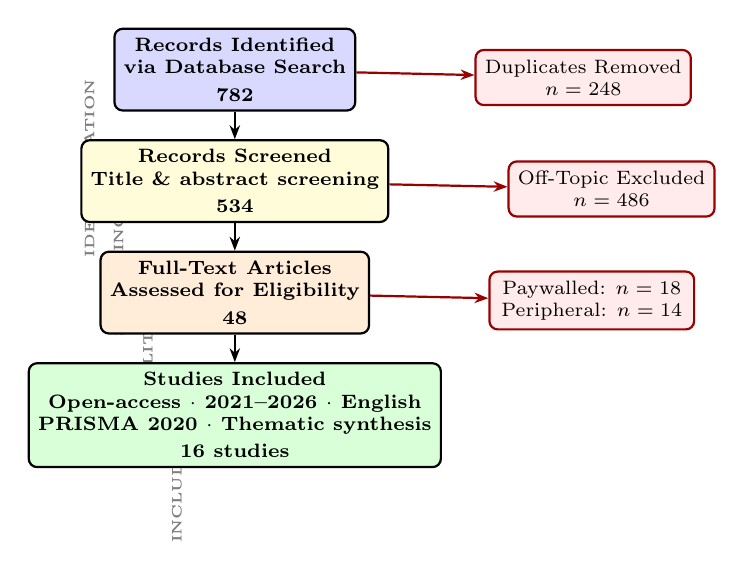
\begin{tikzpicture}[node distance=0.45cm and 1.6cm]

%% Left column: stage labels
\node[font=\tiny\bfseries, rotate=90, text=gray] (idlabel)  {IDENTIFICATION};
\node[font=\tiny\bfseries, rotate=90, text=gray, below=1.35cm of idlabel] (sclabel)  {SCREENING};
\node[font=\tiny\bfseries, rotate=90, text=gray, below=1.35cm of sclabel] (ellabel)  {ELIGIBILITY};
\node[font=\tiny\bfseries, rotate=90, text=gray, below=1.35cm of ellabel] (inclabel) {INCLUDED};

%% Main flow boxes (right of labels)
\node[prismabox=blue, right=0.3cm of idlabel, yshift=0cm]
  (id) {Records Identified\\via Database Search\\[2pt]\textbf{782}};

\node[prismabox=yellow, below=0.35cm of id]
  (sc) {Records Screened\\Title \& abstract screening\\[2pt]\textbf{534}};

\node[prismabox=orange, below=0.35cm of sc]
  (el) {Full-Text Articles\\Assessed for Eligibility\\[2pt]\textbf{48}};

\node[prismabox=green, below=0.35cm of el]
  (inc) {Studies Included\\Open-access $\cdot$ 2021--2026 $\cdot$ English\\PRISMA 2020 $\cdot$ Thematic synthesis\\[2pt]\textbf{16 studies}};

%% Exclusion boxes (right)
\node[excludebox, right=1.5cm of id, yshift=-0.1cm]
  (dup) {Duplicates Removed\\$n = 248$};

\node[excludebox, right=1.5cm of sc, yshift=-0.1cm]
  (offt) {Off-Topic Excluded\\$n = 486$};

\node[excludebox, right=1.5cm of el, yshift=-0.1cm]
  (excl) {Paywalled: $n=18$\\Peripheral: $n=14$};

%% Arrows main flow
\draw[arrow] (id)  -- (sc);
\draw[arrow] (sc)  -- (el);
\draw[arrow] (el)  -- (inc);

%% Arrows to exclusions
\draw[arrow, draw=red!60!black] (id) -- (dup);
\draw[arrow, draw=red!60!black] (sc) -- (offt);
\draw[arrow, draw=red!60!black] (el) -- (excl);

\end{tikzpicture}
\caption{PRISMA 2020 literature selection flow: 782 records identified;
16 studies included after duplicate removal, screening, and eligibility
assessment.}
\label{fig:prisma}
\end{figure}

%% ── Fig 2: Five-phase methodology ────────────────────────────────────────
\begin{figure}[t]
\centering
\begin{tikzpicture}[node distance=0.3cm]

\def\phases{%
  {blue}  / {1} / {Protocol Design \& Research Question Formulation}  /
    {Pre-registration of systematic review protocol $\cdot$ RQs 1--4 formally defined $\cdot$ Database list, query strings \& eligibility criteria established $\cdot$ Scope: cloud forensics challenge landscape in Bangladesh},
  {cyan!60!blue} / {2} / {Multi-Database Systematic Search} /
    {7 repositories: arXiv $\cdot$ MDPI $\cdot$ Google Scholar $\cdot$ SSRN $\cdot$ NDC $\cdot$ BJMIS $\cdot$ IJRIAS $\cdot$ Consistent query applied $\cdot$ $n = 782$ records retrieved},
  {orange!80!red} / {3} / {PRISMA 2020 Screening \& Eligibility Assessment} /
    {Stage 1: Title/abstract screening $n=534$ $\cdot$ Stage 2: Full-text review $n=48$ $\cdot$ Excluded: 32 (paywalled=18, peripheral=14) $\cdot$ Final: 16 studies (2021--2026, open-access)},
  {violet} / {4} / {Thematic Synthesis Across 5 Challenge Clusters} /
    {C1 Volatile Data \& Log Expiry $\cdot$ C2 Multi-Tenancy \& Evidence Contamination $\cdot$ C3 Chain-of-Custody \& s.65B $\cdot$ C4 Cross-Border Jurisdiction \& MLAT Latency $\cdot$ C5 Forensic Readiness Deficit},
  {teal}   / {5} / {AI-Enhanced Solution Mapping \& Framework Synthesis} /
    {Each challenge cluster mapped to validated AI/automation tool $\cdot$ Output: AI-CFRF-BD 5-cluster 5-solution framework $\cdot$ Phased implementation pathway for BD law enforcement \& policymakers}%
}

\foreach \col/\num/\title/\detail [count=\i] in \phases {
  \node[phasebox=\col,
        below=\pgflinewidth of \pgfpicturebbox.south,  % stacked tight
        anchor=north]
    at ($(0, -\i*1.55cm + 1.55cm)$)
    (phase\num) {%
      \begin{minipage}{5.6cm}
        \raggedright
        {\color{\col!80!black}\bfseries Phase \num~---~\title}\\[2pt]
        \tiny\detail
      \end{minipage}};
  \node[phasenum=\col, left=0.18cm of phase\num.west, anchor=east] {\num};
}

\end{tikzpicture}
\caption{Five-phase research methodology: protocol design, multi-database
search, PRISMA screening, thematic synthesis, and AI-enhanced solution
mapping.}
\label{fig:phases}
\end{figure}

\subsection{Inclusion and Exclusion Criteria}

A paper was included if it met four conditions: it addressed at least one
of the five challenge dimensions derived from RQ1 and RQ2; it was
published between 2021 and 2026; it was available in full text without a
paywall; and it was in English. The paywall criterion deserves a brief
note. This review is itself open-access, and including paywalled sources
would undermine reproducibility---readers checking the synthesis against
the cited papers should be able to read those papers. Papers were
excluded if they addressed only physical-device forensics without
touching on the cloud context, or if they were conference abstracts
lacking a methodology section. The latter exclusion is conservative but
defensible: abstracts do not provide enough information to assess the
quality of the underlying work.

\subsection{PRISMA Screening Process}

Of 782 initial records, 248 duplicates were removed. Screening the
remaining 534 records by title and abstract, we excluded 486 as outside
scope. The 48 full-text papers were read in full: 18 were paywalled, and
14 proved too tangentially connected to any of the five clusters to
justify inclusion. The final 16 studies are all open-access, span
2021--2026, and each addresses at least one challenge dimension directly.
Fig.~\ref{fig:prisma} shows the full flow.

\subsection{Thematic Synthesis and Framework Construction}

A single reviewer coded all 16 studies using the thematic synthesis
procedure of Thomas and Harden~\cite{thomas2008}; the absence of
inter-rater verification is a stated limitation. Each study was coded on
three dimensions: (a) which challenge cluster(s) it addresses; (b)
whether Bangladesh relevance is direct, partial, or absent; and (c)
whether it proposes an AI or automation-based resolution tool. The
comparative matrix is in Table~\ref{tab:comparison}. We then matched
each cluster to the highest-evidenced resolution tool (RQ3) based on
empirical metrics---F1-scores, jurisdiction counts, and latency and cost
reductions---yielding the AI-CFRF-BD framework (RQ4).
Table~\ref{tab:taxonomy} presents the complete taxonomy.

%% ── Table I: Comparative analysis ────────────────────────────────────────
\begin{table*}[t]
\caption{Comparative Analysis of Most Relevant Prior Studies Against the
         Five Challenge Dimensions}
\label{tab:comparison}
\small
\begin{tabularx}{\textwidth}{@{} l X c c c c c c c l l @{}}
\toprule
\textbf{Ref} & \textbf{Focus \& Contribution}
  & \textbf{C1} & \textbf{C2} & \textbf{C3} & \textbf{C4} & \textbf{C5}
  & \textbf{AI Tech.} & \textbf{BD Rel.} & \textbf{Method} & \textbf{Year} \\
\midrule
\cite{alshabibi2024} & Alshabibi et al.\ --- SLR, 7 tech.\ + 5 legal barriers
  & $\checkmark$ & $\checkmark$ & $\blacksquare$ & $\blacksquare$ & $\checkmark$
  & ML survey & $\times$ & SLR & 2024 \\
\cite{alharthi2025}  & Alharthi \& Garcia --- CIAF LLM (93\% F1)
  & $\checkmark$ & $\checkmark$ & $\blacksquare$ & $\times$ & $\blacksquare$
  & LLM/GenAI & $\blacksquare$ & Framework & 2025 \\
\cite{igonor2025}    & Igonor et al.\ --- blockchain CoC, 14/17 jurisd.\
  & $\times$ & $\blacksquare$ & $\checkmark$ & $\checkmark$ & $\times$
  & Blockchain & $\blacksquare$ & Prototype & 2025 \\
\cite{tageldin2023}  & Tageldin \& Venter --- ML-CF, ISO/IEC~27043
  & $\checkmark$ & $\checkmark$ & $\blacksquare$ & $\times$ & $\checkmark$
  & ML/LSTM & $\blacksquare$ & SLR & 2023 \\
\cite{akilal2025}    & Akilal \& Kechadi --- CLERMS, 40--70\% MLAT
  & $\checkmark$ & $\times$ & $\times$ & $\checkmark$ & $\blacksquare$
  & NLP/Log & $\blacksquare$ & Prototype & 2025 \\
\cite{ahmed2025}     & Ahmed \& Arifuzzaman --- CSA~2023 BD gap
  & $\checkmark$ & $\checkmark$ & $\checkmark$ & $\blacksquare$ & $\checkmark$
  & Statistical & $\checkmark$ & Survey & 2025 \\
\cite{akter2023}     & Akter \& Rahman --- cloud forensic dims., UIU
  & $\checkmark$ & $\checkmark$ & $\checkmark$ & $\checkmark$ & $\blacksquare$
  & Process ML & $\checkmark$ & SLR+Model & 2023 \\
\cite{sharmin2025}   & Sharmin \& Rahman --- BD Police survey (52)
  & $\blacksquare$ & $\times$ & $\checkmark$ & $\checkmark$ & $\checkmark$
  & Statistical & $\checkmark$ & Survey & 2025 \\
\textbf{[P]}         & \textbf{This study --- AI-CFRF-BD (PRISMA SLR)}
  & $\checkmark$ & $\checkmark$ & $\checkmark$ & $\checkmark$ & $\checkmark$
  & LLM+ML+BC & $\checkmark$ & PRISMA & 2026 \\
\bottomrule
\multicolumn{11}{@{}l@{}}{\footnotesize
  $\checkmark$ = Fully addressed \quad $\blacksquare$ = Partially \quad
  $\times$ = Not addressed \quad BD Rel. = Bangladesh relevance \quad
  [P] = This study}
\end{tabularx}
\end{table*}

%% ── Table II: Taxonomy ────────────────────────────────────────────────────
\begin{table*}[t]
\caption{Taxonomy of Cloud Forensics Challenges, AI Solutions, and Bangladesh Context}
\label{tab:taxonomy}
\small
\begin{tabularx}{\textwidth}{@{} c p{2.6cm} p{3.0cm} p{3.5cm} p{2.8cm} c @{}}
\toprule
\textbf{ID} & \textbf{Challenge \& Root Cause}
            & \textbf{BD Legal Gap}
            & \textbf{AI Resolution Tool}
            & \textbf{BD Impact Metric}
            & \textbf{Metric} \\
\midrule
C1 & Volatile Data \& Log Expiry. CSP logs auto-deleted (30--90 days);
     detection window closes before court order issues.
   & No data-hold statute; ICT Act 2006 \& CSA~2023 silent.
   & CIAF \cite{alharthi2025}: LLM hash-stamps logs before deletion;
     no CSP cooperation required.
   & Evidence stamped in window; no legislative change; deploys with NTMC.
   & 93\% F1 \\
\midrule
C2 & Multi-Tenancy \& Evidence Contamination. Shared infra; container
     isolation weak; one tenant extraction risks co-resident exposure.
   & BD criminal code silent on commingled evidence; CSA~2023 does not
     address this.
   & ML-CF \cite{tageldin2023}: RF, LSTM, CNN isolate forensic artefacts;
     ISO/IEC~27043-aligned.
   & Artefacts from NTMC feeds; no new legislation; ISO/IEC~27043 aligned.
   & ISO/IEC 27043 \\
\midrule
C3 & Chain-of-Custody \& s.65B Admissibility. No CSP-to-court custody
     record; s.65B drafted for physical devices.
   & s.65B precondition unmet for cloud logs; no MoL blockchain guidance;
     Tribunal acquittals \cite{uzzal2025}.
   & Blockchain CoC \cite{igonor2025}: Smart-contracts hash + timestamp
     each custody step.
   & Admissible s.65B; MoL note suffices; no single-custodian trust.
   & 14/17 jurisdictions \\
\midrule
C4 & Cross-Border MLAT Latency. MLAT delays 6\,wk--10\,mo; BD:
     $<$50/yr; Budapest Convention not ratified.
   & No US/EU CSP data-sharing; no specialist digital evidence track
     in MLAT.
   & CLERMS \cite{akilal2025}: NLP pre-validates MLAT requests; catches
     errors pre-submission.
   & Low-cost MoFA/MoL change; faster preservation; fewer wasted requests.
   & 40--70\% MLAT reduction \\
\midrule
C5 & Forensic Readiness Deficit. No pre-incident logging; reactive
     posture; endpoint tools; primary logs never captured.
   & BTRC \& CSA~2023 impose no logging standard or pre-incident config
     in BD.
   & Self-Hosted CF \cite{selfhosted2025}: NTMC integration; no CSP
     cooperation; existing intercept authority.
   & Pre-incident capture; within legal authority; reduces investigation
     costs.
   & 60\% cost reduction \\
\bottomrule
\multicolumn{6}{@{}l@{}}{\footnotesize
  CIAF = Cloud Intelligence \& AI Forensics; CoC = Chain of Custody;
  MoL = Ministry of Law; CLERMS = Cross-border LE Req.\ Mgmt.;
  MoFA = Min.\ Foreign Affairs; NTMC = Nat'l Telecom Mon.\ Ctr.}
\end{tabularx}
\end{table*}

%% ══════════════════════════════════════════════════════════════════════════
\balance
\bibliographystyle{ACM-Reference-Format}
\begin{thebibliography}{19}

\bibitem{alshabibi2024}
A.~Alshabibi, P.~Liatsis, and A.~Emhemed,
``Cloud forensic investigation challenges: A systematic literature review,''
\textit{Computers}, vol.~13, no.~8, p.~213, Aug.~2024.
\newblock \url{https://doi.org/10.3390/computers13080213}

\bibitem{alenezi2023}
M.~Alenezi,
``Cloud forensics challenges: A technical and legal taxonomy,''
\textit{arXiv}:2305.03059, May~2023.

\bibitem{prakash2021}
A.~Prakash, A.~V.~Srivastava, and R.~Gupta,
``Forensic investigation in cloud and edge computing environments,''
\textit{Electronics}, vol.~10, no.~11, p.~1229, 2021.
\newblock \url{https://doi.org/10.3390/electronics10111229}

\bibitem{selfhosted2025}
``Self-hosted cloud forensics: An open-source framework for evidence
acquisition,''
\textit{arXiv}:2510.21246v2, 2025.

\bibitem{alharthi2025}
B.~S.~Alharthi and L.~F.~Garcia,
``Cloud intelligence and AI forensics (CIAF): Large language models for
automated cloud forensics,''
\textit{arXiv}:2510.00452, Oct.~2025.

\bibitem{igonor2025}
A.~Igonor, A.~Nweke, O.~Adigwe, and V.~Ahiwe,
``A systematic review of blockchain technology for digital forensics,''
\textit{Blockchains}, vol.~3, no.~1, p.~5, 2025.
\newblock \url{https://doi.org/10.3390/blockchains3010005}

\bibitem{tageldin2023}
M.~Tageldin and H.~S.~Venter,
``Proposing a machine learning-based cloud forensics investigation
framework,''
\textit{Applied Sciences}, vol.~13, no.~18, p.~10169, 2023.
\newblock \url{https://doi.org/10.3390/app131810169}

\bibitem{karagiannis2021}
S.~Karagiannis and E.~Vergidis,
``Digital evidence and cloud forensics: Contemporary legal challenges and
prospects,''
\textit{Information}, vol.~12, no.~5, p.~181, 2021.
\newblock \url{https://doi.org/10.3390/info12050181}

\bibitem{akilal2025}
M.~Akilal and M.-T.~Kechadi,
``A cross-border law enforcement request management system (CLERMS) for
digital forensics,''
\textit{arXiv}:2507.04174, Jul.~2025.

\bibitem{ali2023}
M.~A.~Ali,
``Digital evidence and cyber crime investigation: Bangladesh perspective,''
\textit{NDC e-Journal}, vol.~22, no.~2, 2023.

\bibitem{uzzal2025}
M.~R.~Uzzal,
``Cybercrime and digital evidence in Bangladesh: A critical analysis,''
SSRN preprint, 2025.
\newblock \url{https://doi.org/10.2139/ssrn.5079527}

\bibitem{ahmed2025}
S.~Ahmed and M.~Arifuzzaman,
``Cyber security law in Bangladesh: A critical analysis of the Cyber
Security Act 2023,''
\textit{Asian J.\ Social Sci.\ Legal Stud.}, vol.~7, no.~4, pp.~347--357, 2025.

\bibitem{akter2023}
S.~S.~Akter and M.~S.~Rahman,
``Cloud forensic: Issues, challenges and solution models,''
in \textit{A Practical Guide on Security and Privacy in Cyber Physical
Systems}. Singapore: World Scientific, 2023.

\bibitem{ekwempu2026}
F.~C.~Ekwempu,
``Investigating the legal complexities of cloud forensic investigations in
cross-border scenarios and developing strategies for international
cooperation,''
\textit{Int.\ J.\ Res.\ Innov.\ Appl.\ Sci.}, vol.~11, no.~1,
pp.~1334--1343, Jan.~2026.
\newblock \url{https://doi.org/10.51584/IJRIAS.2026.110100113}

\bibitem{sharmin2025}
K.~Sharmin and I.~M.~Rahman,
``Digital forensics empowerment of Bangladesh police: A comprehensive
analysis of its role in preventing crimes and enhancing investigative
capabilities,''
\textit{Bangladesh J.\ MIS}, vol.~11, no.~1, 2025.
\newblock \url{https://doi.org/10.61606/BJMIS.V11N1.A1}

\bibitem{rana2025}
M.~S.~Rana,
``Criminal investigation in the digital era: Lessons for Bangladesh from
Colombia, India, and the United States,''
\textit{Conhecimento \& Diversidade}, vol.~17, no.~47, pp.~91--107,
Jul.--Sep.~2025.

\bibitem{thomas2008}
J.~Thomas and A.~Harden,
``Methods for the thematic synthesis of qualitative research in systematic
reviews,''
\textit{BMC Med.\ Res.\ Methodol.}, vol.~8, p.~45, 2008.
\newblock \url{https://doi.org/10.1186/1471-2288-8-45}

\bibitem{page2021}
M.~J.~Page et~al.,
``The PRISMA 2020 statement: An updated guideline for reporting systematic
reviews,''
\textit{BMJ}, vol.~372, p.~n71, Mar.~2021.
\newblock \url{https://doi.org/10.1136/bmj.n71}

\bibitem{iso27037}
International Organization for Standardization,
\textit{ISO/IEC~27037:2012 --- Information Technology: Security Techniques
--- Guidelines for Identification, Collection, Acquisition and Preservation
of Digital Evidence}.
Geneva, Switzerland: ISO, 2012.

\end{thebibliography}

\end{document}
